\documentclass[usletter]{article}
\usepackage{amsthm}
\usepackage{mathtools}
\usepackage{multicol}

\usepackage{hw}
\usepackage[margin=1.5in]{geometry}
\usepackage{comment}
\usepackage{url}
\usepackage{enumitem}

\usepackage{tikz}
\usetikzlibrary{automata, positioning}
\usetikzlibrary{arrows}

\begin{document}

\makeheader{First \& Last Name}	% your name
           {100-200-300}          		% your university id
           {02}                     			% unused
           {Regularities, DFA Minimization, and Decidability}	% lecture title

\noindent

\begin{itemize}
\item 100\% = Problem \ref{p1} ($30\%$) + Problem \ref{p2} ($20\%$) + Problem \ref{p3} ($20\%$) + Problem \ref{p4} ($30\%$)
\item Homework 1 is due no later than Thursday 07/28/2016 23:55 as a file on \url{ccle.ucla.edu}, or submitted at the discussion section on a paper
\item Homework file can be in \LaTeX\ (template to be given) or Microsoft Word
%\item Have a question? \url{piazza.com/ucla/summer2016/cs181}
\end{itemize}

%\newpage

\bigskip
\begin{problem}
\label{p1}

(30 pts) For each of the languages below, find whether it is regular or not? Prove that your answer is correct.

\begin{enumerate}[label=(\alph*)]
\item $L_1=\big\{ 1^ky\ |\ y \in \{0,1\}^* \text{ and } y \text{ contains at least } k\ 1\text{s, for all } k\ge 1 \big\}$
\item $L_1=\big\{ 1^ky\ |\ y \in \{0,1\}^* \text{ and } y \text{ contains at most } k\ 1\text{s, for all } k\ge 1 \big\}$
\item $L_3=\big\{ 1^k0y\ |\ y \in \{0,1\}^* \text{ and } y \text{ contains at least } k\ 1\text{s, for all } k\ge 1 \big\}$
\end{enumerate}

\end{problem}

\begin{answer}for Problem \ref{p1}:
%Solution goes here.
\end{answer}











\bigskip
\begin{problem}
\label{p2}

(20 pts) For each of the languages below, find whether it is regular or context free or neither? Prove that your answer is correct.

\begin{enumerate}[label=(\alph*)]
\item $L_4=\big\{ a^{3m}b^2c^m\ |\ m\ge 0 \big\}$
\item $L_5=\big\{ a^{3m}b^2c^n\ |\ n,m\ge 0 \big\}$
\end{enumerate}

\end{problem}

\begin{answer}for Problem \ref{p2}:
%Solution goes here.
\end{answer}







\bigskip
\begin{problem}
\label{p3}
(20 pts) Convert the following NFA to DFA and minimize:

\begin{center}
	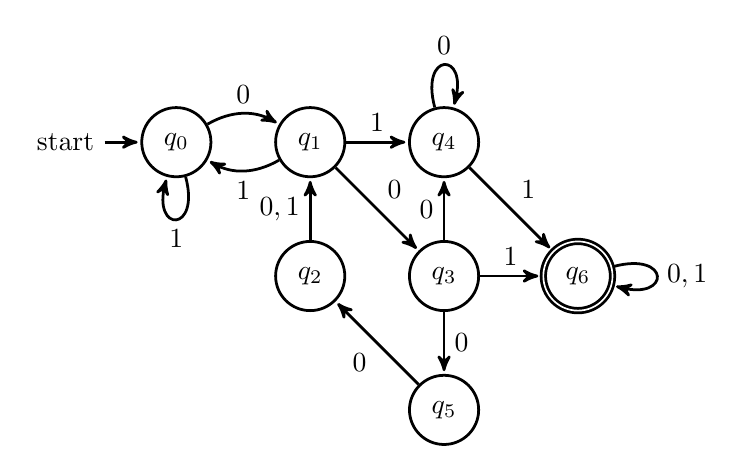
\begin{tikzpicture}[node distance=17mm, auto, line width=1pt, ->,>=stealth',shorten >=1pt]
	\node[state,initial]   		(sq0)                  		{$q_0$};
	\node[state         ]   		(sq1)  [right of=sq0]  		{$q_1$};
	\node[state         ]   		(sq2)  [below of=sq1]		{$q_2$};
	\node[state         ]   		(sq4)  [right of=sq1] {$q_4$};
	\node[state         ]   		(sq3)  [right of=sq2] 		{$q_3$};
	\node[state         ]   		(sq5)  [below of=sq3] 	{$q_5$};
	\node[state,accepting]   	(sq6)  [right of=sq3]  		{$q_6$};
	
	\path[->, line width=1pt, ->,>=stealth',shorten >=1pt] 	
			(sq0) edge[loop below]	node {$1$} ()
			(sq0) edge[bend left] 	node {$0$} 	(sq1)
			(sq1) edge[bend left] 	node {$1$} 	(sq0)
			(sq2) edge[]  			node {$0,1$} 	(sq1)			
			(sq1) edge[]  			node {$0$} 	(sq3)
			(sq3) edge[] 			node {$0$} 	(sq4)
			(sq3) edge[]  			node {$1$} 	(sq6)
			(sq4) edge[]  			node {$1$} 	(sq6)
			(sq3) edge[]  			node {$0$} 	(sq5)
			(sq5) edge[]  			node {$0$} 	(sq2)
			(sq1) edge[]  			node {$1$} 	(sq4)
			(sq4) edge[loop above]  	node {$0$} 	(sq4)
			(sq6) edge[loop right]  	node {$0,1$} 	(sq6)
			;
	\end{tikzpicture}
\end{center}


\end{problem}

\begin{answer}for Problem \ref{p3}:
%Solution goes here.
\end{answer}



















\bigskip
\begin{problem}
\label{p4}
(30 pts) Find if the following problem is algorithmically decidable and prove that your answer is correct:

\begin{quote}
Given three regular languages $L_1$, $L_2$, and $L_3$ in an alphabet $\Sigma$, find if: $$L_1 \cap L_2 \subseteq L_3$$
\end{quote}

\end{problem}

\begin{answer}for Problem \ref{p4}:
%Solution goes here.
\end{answer}

\bibliographystyle{abbrv}
\bibliography{template}

\end{document}
